\title{Travelling Salesman Problem}
\author{Names}
\date{\today}

\documentclass[14pt, english]{article}

\usepackage[T1]{fontenc}
\usepackage{babel}
\usepackage{geometry}
\usepackage{titling}
\usepackage{blindtext}
\usepackage[utf8]{inputenc}
\usepackage{graphicx}
\setlength{\droptitle}{-4em}     % Eliminate the default vertical space
\addtolength{\droptitle}{-4pt}   % Only a guess. Use this for adjustment

\begin{document}
\maketitle
\newcommand\tab[1][1.2cm]{\hspace*{#1}}
\section{Introduction}

Consider a salesman who has to visit a set of cities and return to the city he started from provided he visitseach city only once.\\
\\
\noindent
The problem is to minimize the total cost or distance of the route. This is known as the Travelling Salesman Problem.\\
\\
\noindent
The problem can be summarised as follows: \\
\\
\tab TSP = $\{(G,f,t)$: $G = (V,E)$ is a complete graph,\\
\tab \tab $f$ is a function $V\times V \rightarrow Z,$\\
\tab \tab $t \in Z,$ \\
\tab \tab $G$ is a graph that contains a travelling salesman tour with costs \tab \tab or distances that does not exceed $t\}$.

\subsection{Symmetric Travelling Salesman Problem}

If in a travelling salesman problem, cost or distance of travelling from city $i$ to city $j$ is equal to the cost or distance of travelling from city $j$, $i.e.$ the cost matrix is symmetric, then the problem is said to be \emph{Symmetric Travelling Salesman Problem}.

\subsection{Asymmetric Travelling Salesman Problem}

If in a travelling salesman problem, cost or distance of travelling from city $i$ to city $j$ can differ from the cost or distance of travelling from city $j$, $i.e.$ the cost matrix is asymmetric, then the problem is said to be \emph{Asymmetric Travelling Salesman Problem}. A real world example could be routes consisting of some one-way roads.

\newpage
\section{Branch and Bound With Adding and Removing Edges}
\subsection{Introduction}
One of the strategies used for searching the solution space is Branch and Bound keep dividing the space into branches. one for solutions containing a given edge and the other for those excluding the given edge. forming a binary tree as follows:
\newline \newline
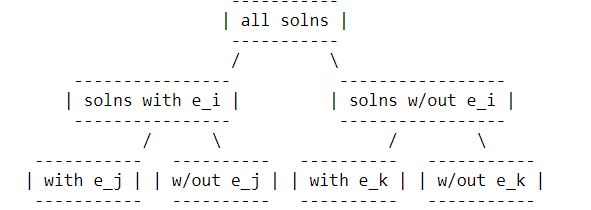
\includegraphics[width=\textwidth] {solution-tree.jpg}
\newline \newline
The main parts of these algorithm are:
\begin{enumerate}
    \item Bounding Function
    \item Choosing Splitting Edge
    \item How to Include Edge
    \item How to Exclude Edge
\end{enumerate}

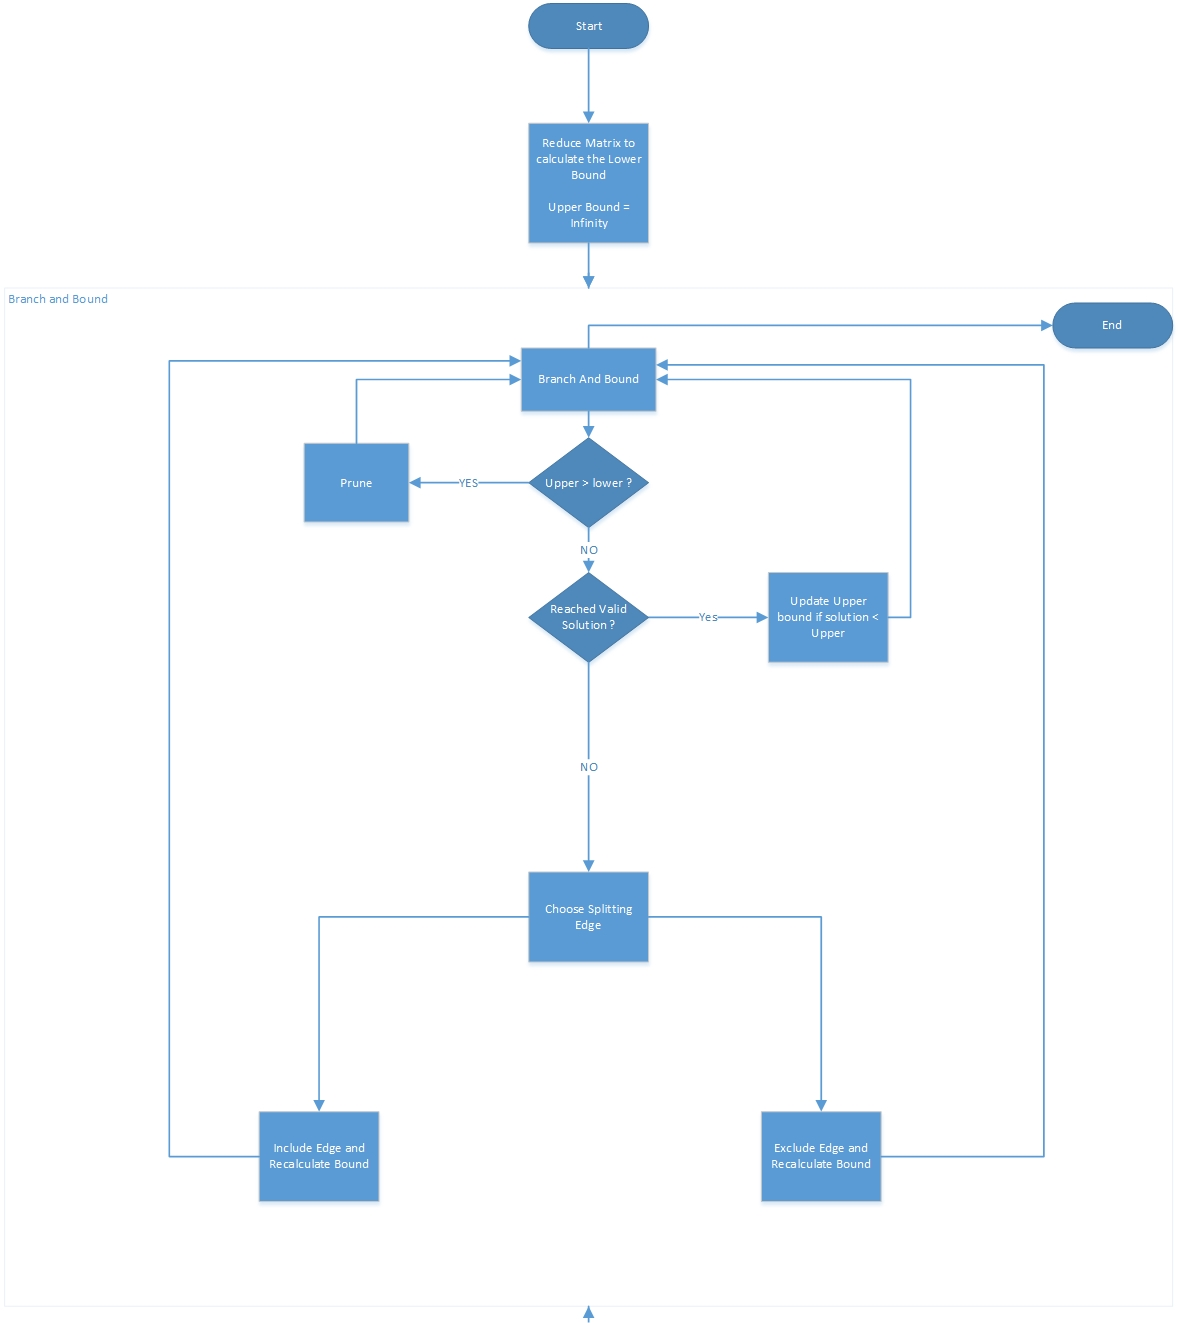
\includegraphics[width = \textwidth]{bnb-flow.jpg}

\newpage
\subsection{Bounding Function (Reduction)}
The solution is bounded by normalizing the solution matrix. this is done by reducing the rows first and the columns after.
by reducing the Rows/Columns we mean normalizing them. we subtract the minimum element from each row from each element at that row. and the same for columns. at the end we will have a matrix with at least one zero in each column and each row.
Our lower bound will be the sum of all minimum values with used to reduce the matrix.

\subsection{Choosing Splitting Edge}
We are looking to maximize the right part by trying to raising the lower bound of the right sub-tree. In order to do that, we choose to split on the edge that best maximize the lower bound. We look for the zero weight edges that maximize the increasing in the lower bound.

\subsection{How to Include Edge}
Including an edge (ie, I -> J) is done by first, forbidding the going back from J -> I by setting the weight of edge J -> to INFINITY ( we also forbid the going back to any sub-path in our partial solution). Moreover, since we have used this edge, we cannot go from node i to any other node, and similarly, we cannot reach node J. Consequently, we delete the I th row and the J th column from our solutions matrix.
in the end, we reduce the new matrix after including the edge.

\subsection{How to Exclude Edge}
To exclude edge (ie, I-> J), we start by setting the cost of the edge I->J to INFINITY. and we reduce the new matrix afterwards.

\section{Genetic Algorithm}
\subsection{Introduction}
We present in this report the main description for the attached source code to solve Travelling salesman Problem. \newline \newline
As illustrated in the figure below, the main algorithm pipeline contains several main components:
\begin{enumerate}
    \item Initializing Algorithm Parameters
    \item Generate Initial Population
    \item Fitness Evaluation
    \item Parents Selection
    \item Crossover
    \item Mutation
    \item Generate New Population
\end{enumerate}
The following sections will explain briefly each components.
\newline \newline
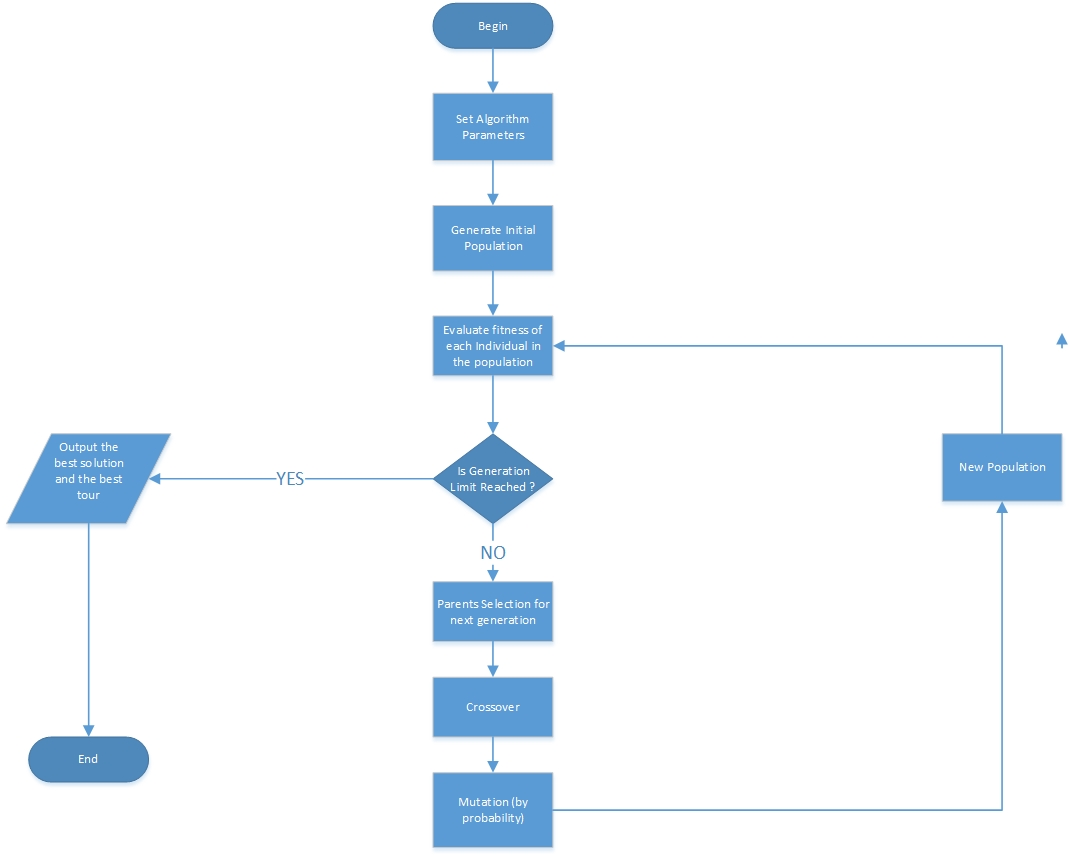
\includegraphics[width=\textwidth]{tsp-genetic-flowchart.jpg}

\subsection{Initializing Algorithm Parameters:}
In this step, several parameters should be initialized by the user. Specifically, \begin{enumerate}
    \item Max Population Size: 
    to specify the maximum number of individuals in any population
    \item Max Generation Numbers: usually the termination condition
    \item Mutation Rate: a real number in [0,1] specify the likelihood of mutation to happen
\end{enumerate}

\subsection{Generate Initial Population:}
In this step an initial generation is created randomly blouiseruthharding
/
tsp_y creating a first random individual (Tour), and use shuffling on this individual until we reach the max population size. 
\subsection{Fitness Evaluation for Elitism:}
in this step, the fitness function for each individual should be calculated. For the TSP problem. the fitness function could be define as the total sum of distances for each tour.
This fitness function is used to evaluate how good each individual (Solution). Consequently, the fittest individual is elited to the next generation directly.
\subsection{Parents Selection:}
In this step, parents are chosen to mate together (crossover) and have a new individual. the selection process could be done in several ways. we applied Roulette Selection (with flexibility in the code to add new other selection algorithms without changing the code).
the basic of Roulette Selection is to pick a parent randomly according to weighted probability for each individual. the weights here represented by the fitness of the individual. In other words, individuals with high fitness function, have higher probabilities to be selected.
\subsection{Crossover:}
The crossover is the process of merging two individuals to have a new ones. there is several ways to implement the crossover. in our case, we implemented the Single Point Crossover. where a random point is generated bounded by the length of the solution. Afterwards, a new individuals are generated by taking the first part (before the picked point) from the first parent and the rest from the other taking into account the satisfaction of TSP constraints (no duplication) 
\subsection{Mutation:}
Each individual might undergo a mutation with a probability (specified in the parameters). the mutation basically is done by scanning the individual genes and picking a random number (bounded by the length of tour) and swap the current gene with the randomly picked one.
\subsection{Generate New Population:}
We keep repeating steps 5,6,7 until we have a full new population (enhanced one). and we go back to step 4 while we have not reached the generation limit.
\end{document}  
